\documentclass[tikz]{standalone}
\usepackage{tikz}
\usetikzlibrary{arrows}

\begin{document}

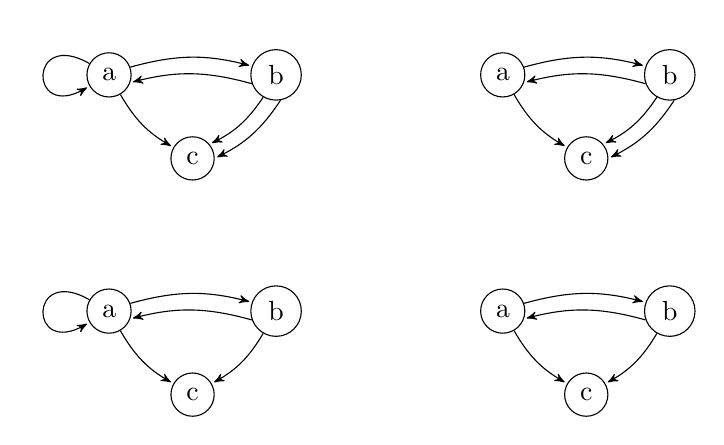
\begin{tikzpicture}[->,>=stealth',shorten >=1pt,auto,node distance=1.5cm,
main node/.style={circle, draw}]

		\node[main node] (c) {c};
		\node[main node] (b) [above right of=c] {b};
		\node[main node] (a) [above left of=c] {a};

		\path[every node/.style={font=\sffamily\small}]
				(a.20) edge [bend left=15] (b.160)
				(b.-160) edge [bend right=15] (a.-20) 
				(a) edge [bend right=15] (c)
				(b.-120) edge [bend left=15] (c.40)
				(b.-80) edge [bend left=15] (c.0)
				(a) edge [out = 150, in = 210, loop] (a);
		
	\begin{scope}[xshift=5cm] 
		
 			\node[main node] (c) {c};
			\node[main node] (b) [above right of=c] {b};
			\node[main node] (a) [above left of=c] {a};

		\path[every node/.style={font=\sffamily\small}]
				(a.20) edge [bend left=15] (b.160)
				(b.-160) edge [bend right=15] (a.-20) 
				(a) edge [bend right=15] (c)
				(b.-120) edge [bend left=15] (c.40)
				(b.-80) edge [bend left=15] (c.0);
				
	\end{scope}	

	\begin{scope}[yshift=-3cm] 
		
 			\node[main node] (c) {c};
			\node[main node] (b) [above right of=c] {b};
			\node[main node] (a) [above left of=c] {a};

		\path[every node/.style={font=\sffamily\small}]
				(a.20) edge [bend left=15] (b.160)
				(b.-160) edge [bend right=15] (a.-20) 
				(a) edge [bend right=15] (c)
				(b) edge [bend left=15] (c)
				(a) edge [out = 150, in = 210, loop] (a);
				
	\end{scope}	

	\begin{scope}[xshift=5cm, yshift=-3cm] 
		
 			\node[main node] (c) {c};
			\node[main node] (b) [above right of=c] {b};
			\node[main node] (a) [above left of=c] {a};

		\path[every node/.style={font=\sffamily\small}]
				(a.20) edge [bend left=15] (b.160)
				(b.-160) edge [bend right=15] (a.-20) 
				(a) edge [bend right=15] (c)
				(b) edge [bend left=15] (c);	
				
	\end{scope}	

\end{tikzpicture}

\end{document}

%%% Local Variables: 
%%% mode: latex
%%% TeX-master: t
%%% End: 
